\section{Compaction triggers and delayed credit}\label{sec:C12:triggers}
A fixed threshold triggers compaction when the current input exceeds a fraction of the window. This is easy to implement and creates predictable resource bounds, but it ignores semantic phase boundaries. Compressing immediately before a decisive action can discard evidence that would have been useful for verification. Compressing after a stable subtask finishes may be less risky because its outcome can be represented as a validated artifact. A trigger should consider both token pressure and the task's transition structure.

For a fixed continuation policy and the same pre-edit history $H_t$, let $C_{t:T}^{(1)}$ and $C_{t:T}^{(0)}$ denote potential continuation costs under editing and retaining the current view, respectively. Both costs include the transformation itself and subsequent repair work. A controller may compare
\begin{equation}
 \Delta_t=\mathbb E\!\left[
 C_{t:T}^{(1)}-C_{t:T}^{(0)}\mid H_t\right].
\end{equation}
Choosing an edit when $\Delta_t<0$ minimizes this local two-action cost only if the estimates are correct, both actions satisfy the outcome and authority constraints, and the horizon captures relevant consequences. Observational averages over previously edited and unedited tasks do not identify this contrast when selection differs. In practice, these estimates are uncertain. A trigger can include a margin that reflects uncertainty, or it can defer compaction until a task checkpoint establishes a stable state. Neither device eliminates the need to test delayed failures.

Reward shaping can help assign local feedback to context actions, but it can also change the optimized behavior. Penalizing context length rewards short inputs even if later repair is expensive. Rewarding successful retrieval can encourage unnecessary retrieval. A better diagnostic records downstream task outcome, semantic information loss, tool interactions, and cumulative cost separately. A scalar training objective may combine them, while the evaluation retains the separate quantities so tradeoffs remain visible.

Counterfactual continuation is particularly informative. Save the environment state before an edit and evaluate continuations with the original view, the edited view, and an edited view augmented with the omitted decisive record. If the third condition repairs a failure, the evidence supports a context-loss mechanism. If it does not, the failure may involve reasoning, environment stochasticity, or a changed action policy. Environment restoration must itself be validated; otherwise the counterfactual comparison changes more than the context.

Training introduces an additional requirement: each generated token must be associated with the context actually visible when it was produced. MemoryWalker identifies conditioning errors when edited rollouts are flattened into a final compressed trace or a full physical history~\cite{j2026memorywalker}. Chapter~\ref{ch:C17} develops the corresponding likelihood contracts. The point for trigger design is that an edit is not only an inference-time event. It changes the data structure required to train correctly on the resulting trajectory.

Practical controllers should therefore emit an edit manifest containing the decision time, removed spans, replacement text, source identifiers, and view version. This manifest supports both failure analysis and correct rollout reconstruction. Recording only the final summary loses the temporal information needed to determine whether a token was trained under a future edit or under content that had already disappeared.



Figure~\ref{fig:C12:paired-context-intervention} isolates the mechanism and its stated information boundaries.
\begin{figure}[!htbp]
\centering
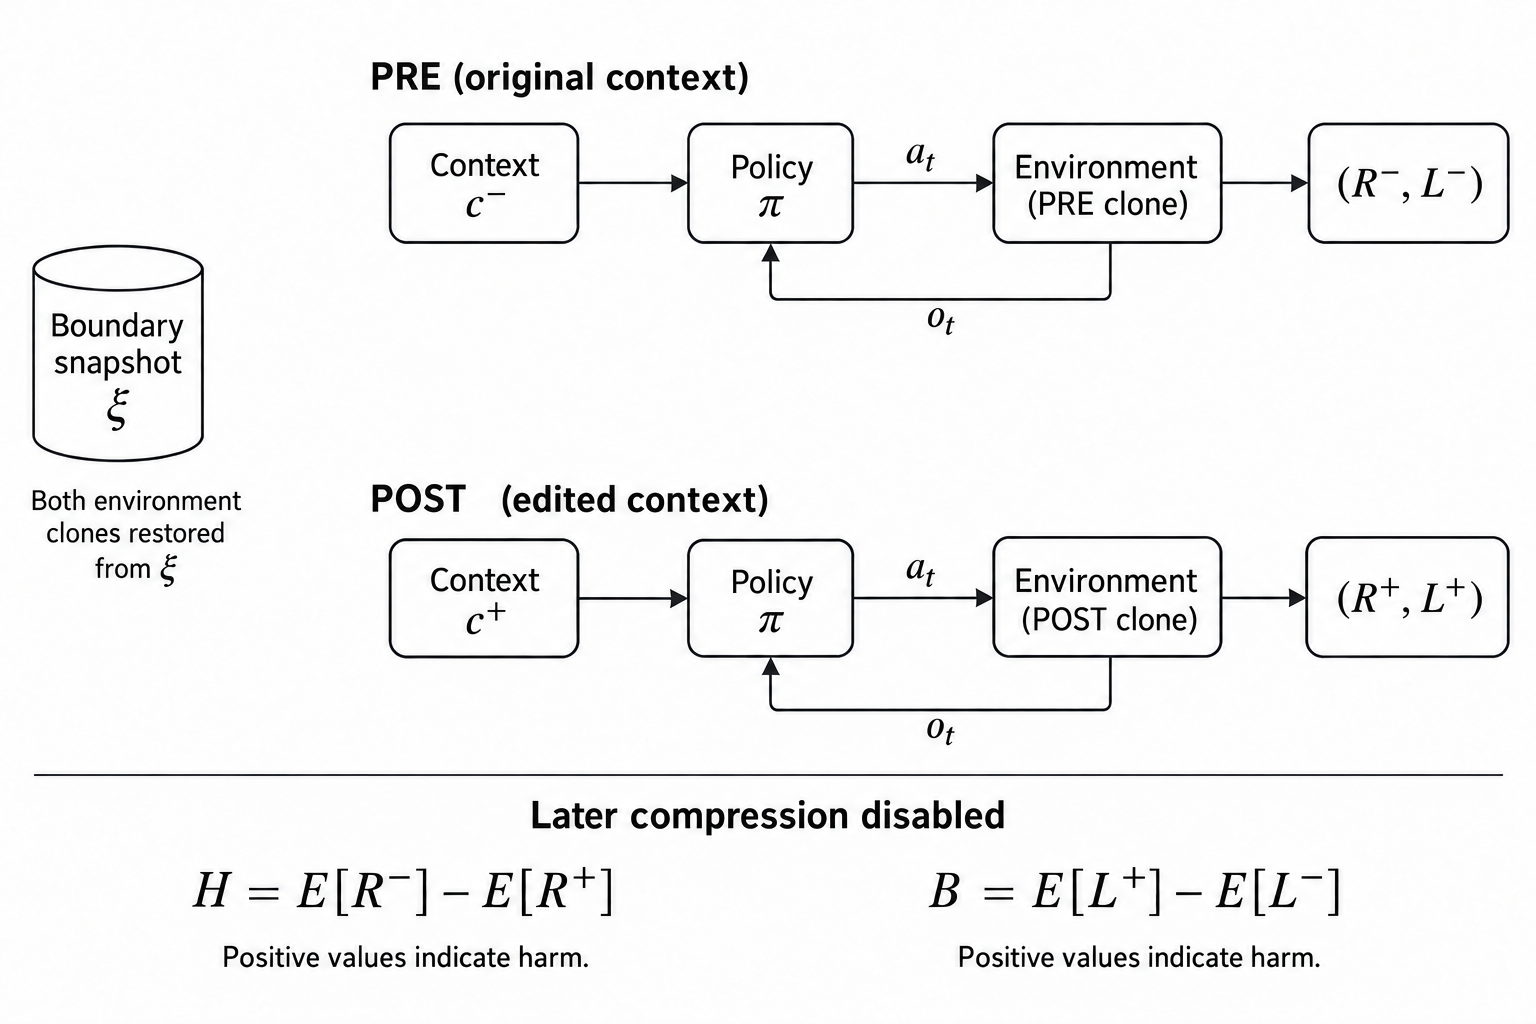
\includegraphics[width=\linewidth]{book/figures/assets/F12review.png}
\caption{A paired continuation diagnostic changes the working view while restoring the same external boundary state and holding the continuation policy fixed. Disabling later compression isolates the current replacement. Outcome hazard $H=\mathbb E[R^-]-\mathbb E[R^+]$ and interaction burden $B=\mathbb E[L^+]-\mathbb E[L^-]$ quantify different consequences. Estimation requires validated restoration and repeated continuations; no outcomes are depicted. Original schematic informed by PAIR~\cite{min2026pair}.}
\label{fig:C12:paired-context-intervention}
\end{figure}
